\documentclass[11pt,ignorenonframetext,]{beamer}
\setbeamertemplate{caption}[numbered]
\setbeamertemplate{caption label separator}{: }
\setbeamercolor{caption name}{fg=normal text.fg}
\beamertemplatenavigationsymbolsempty
\usepackage{lmodern}
\usepackage{amssymb,amsmath}
\usepackage{ifxetex,ifluatex}
\usepackage{fixltx2e} % provides \textsubscript
\ifnum 0\ifxetex 1\fi\ifluatex 1\fi=0 % if pdftex
  \usepackage[T1]{fontenc}
  \usepackage[utf8]{inputenc}
\else % if luatex or xelatex
  \ifxetex
    \usepackage{mathspec}
  \else
    \usepackage{fontspec}
  \fi
  \defaultfontfeatures{Ligatures=TeX,Scale=MatchLowercase}
\fi
\usetheme[]{metropolis}
% use upquote if available, for straight quotes in verbatim environments
\IfFileExists{upquote.sty}{\usepackage{upquote}}{}
% use microtype if available
\IfFileExists{microtype.sty}{%
\usepackage{microtype}
\UseMicrotypeSet[protrusion]{basicmath} % disable protrusion for tt fonts
}{}
\newif\ifbibliography
\hypersetup{
            pdftitle={Lecture 11},
            pdfauthor={Colin Rundel},
            pdfborder={0 0 0},
            breaklinks=true}
\urlstyle{same}  % don't use monospace font for urls
\usepackage{color}
\usepackage{fancyvrb}
\newcommand{\VerbBar}{|}
\newcommand{\VERB}{\Verb[commandchars=\\\{\}]}
\DefineVerbatimEnvironment{Highlighting}{Verbatim}{commandchars=\\\{\}}
% Add ',fontsize=\small' for more characters per line
\newenvironment{Shaded}{}{}
\newcommand{\KeywordTok}[1]{\textcolor[rgb]{0.00,0.44,0.13}{\textbf{#1}}}
\newcommand{\DataTypeTok}[1]{\textcolor[rgb]{0.56,0.13,0.00}{#1}}
\newcommand{\DecValTok}[1]{\textcolor[rgb]{0.25,0.63,0.44}{#1}}
\newcommand{\BaseNTok}[1]{\textcolor[rgb]{0.25,0.63,0.44}{#1}}
\newcommand{\FloatTok}[1]{\textcolor[rgb]{0.25,0.63,0.44}{#1}}
\newcommand{\ConstantTok}[1]{\textcolor[rgb]{0.53,0.00,0.00}{#1}}
\newcommand{\CharTok}[1]{\textcolor[rgb]{0.25,0.44,0.63}{#1}}
\newcommand{\SpecialCharTok}[1]{\textcolor[rgb]{0.25,0.44,0.63}{#1}}
\newcommand{\StringTok}[1]{\textcolor[rgb]{0.25,0.44,0.63}{#1}}
\newcommand{\VerbatimStringTok}[1]{\textcolor[rgb]{0.25,0.44,0.63}{#1}}
\newcommand{\SpecialStringTok}[1]{\textcolor[rgb]{0.73,0.40,0.53}{#1}}
\newcommand{\ImportTok}[1]{#1}
\newcommand{\CommentTok}[1]{\textcolor[rgb]{0.38,0.63,0.69}{\textit{#1}}}
\newcommand{\DocumentationTok}[1]{\textcolor[rgb]{0.73,0.13,0.13}{\textit{#1}}}
\newcommand{\AnnotationTok}[1]{\textcolor[rgb]{0.38,0.63,0.69}{\textbf{\textit{#1}}}}
\newcommand{\CommentVarTok}[1]{\textcolor[rgb]{0.38,0.63,0.69}{\textbf{\textit{#1}}}}
\newcommand{\OtherTok}[1]{\textcolor[rgb]{0.00,0.44,0.13}{#1}}
\newcommand{\FunctionTok}[1]{\textcolor[rgb]{0.02,0.16,0.49}{#1}}
\newcommand{\VariableTok}[1]{\textcolor[rgb]{0.10,0.09,0.49}{#1}}
\newcommand{\ControlFlowTok}[1]{\textcolor[rgb]{0.00,0.44,0.13}{\textbf{#1}}}
\newcommand{\OperatorTok}[1]{\textcolor[rgb]{0.40,0.40,0.40}{#1}}
\newcommand{\BuiltInTok}[1]{#1}
\newcommand{\ExtensionTok}[1]{#1}
\newcommand{\PreprocessorTok}[1]{\textcolor[rgb]{0.74,0.48,0.00}{#1}}
\newcommand{\AttributeTok}[1]{\textcolor[rgb]{0.49,0.56,0.16}{#1}}
\newcommand{\RegionMarkerTok}[1]{#1}
\newcommand{\InformationTok}[1]{\textcolor[rgb]{0.38,0.63,0.69}{\textbf{\textit{#1}}}}
\newcommand{\WarningTok}[1]{\textcolor[rgb]{0.38,0.63,0.69}{\textbf{\textit{#1}}}}
\newcommand{\AlertTok}[1]{\textcolor[rgb]{1.00,0.00,0.00}{\textbf{#1}}}
\newcommand{\ErrorTok}[1]{\textcolor[rgb]{1.00,0.00,0.00}{\textbf{#1}}}
\newcommand{\NormalTok}[1]{#1}
\usepackage{graphicx,grffile}
\makeatletter
\def\maxwidth{\ifdim\Gin@nat@width>\linewidth\linewidth\else\Gin@nat@width\fi}
\def\maxheight{\ifdim\Gin@nat@height>\textheight0.8\textheight\else\Gin@nat@height\fi}
\makeatother
% Scale images if necessary, so that they will not overflow the page
% margins by default, and it is still possible to overwrite the defaults
% using explicit options in \includegraphics[width, height, ...]{}
\setkeys{Gin}{width=\maxwidth,height=\maxheight,keepaspectratio}

% Prevent slide breaks in the middle of a paragraph:
\widowpenalties 1 10000
\raggedbottom

\AtBeginPart{
  \let\insertpartnumber\relax
  \let\partname\relax
  \frame{\partpage}
}
\AtBeginSection{
  \ifbibliography
  \else
    \let\insertsectionnumber\relax
    \let\sectionname\relax
    \frame{\sectionpage}
  \fi
}
\AtBeginSubsection{
  \let\insertsubsectionnumber\relax
  \let\subsectionname\relax
  \frame{\subsectionpage}
}

\setlength{\parindent}{0pt}
\setlength{\parskip}{6pt plus 2pt minus 1pt}
\setlength{\emergencystretch}{3em}  % prevent overfull lines
\providecommand{\tightlist}{%
  \setlength{\itemsep}{0pt}\setlength{\parskip}{0pt}}
\setcounter{secnumdepth}{0}

\usepackage{geometry}
\usepackage{graphicx}
\usepackage{amssymb}
\usepackage{color}          	% gives color options
\usepackage{url}		% produces hyperlinks
\usepackage[english]{babel}
\usepackage{colortbl}	% allows for color usage in tables
\usepackage{multirow}	% allows for rows that span multiple rows in tables
\usepackage{xcolor}		% this package has a variety of color options
\usepackage{calc}
\usepackage{multicol}
\usepackage{wrapfig}
\usepackage{textcomp}
\usepackage{bm}
\usepackage{bbm}
\usepackage{setspace}
\singlespacing

%%%%%%%%%%%%%%%%
% Small code output
%%%%%%%%%%%%%%%%

%% change fontsize of R code

\makeatletter
\@ifundefined{Shaded}{\newenvironment{Shaded}{}{}}{}
\makeatother


\let\oldShaded\Shaded
\let\endoldShaded\endShaded
\renewenvironment{Shaded}{\footnotesize\begin{spacing}{0.9}\oldShaded}{\endoldShaded\end{spacing}}

%% change fontsize of output
\let\oldverbatim\verbatim
\let\endoldverbatim\endverbatim
\renewenvironment{verbatim}{\footnotesize\begin{spacing}{0.9}\oldverbatim}{\endoldverbatim\end{spacing}}


\newcommand{\tinyoutput}{
  \renewenvironment{Shaded}{\tiny\begin{spacing}{0.9}\oldShaded}{\endoldShaded\end{spacing}}
  \renewenvironment{verbatim}{\tiny\begin{spacing}{0.9}\oldverbatim}{\endoldverbatim\end{spacing}}
}

\newcommand{\scriptoutput}{
  \renewenvironment{Shaded}{\scriptsize\begin{spacing}{0.9}\oldShaded}{\endoldShaded\end{spacing}}
  \renewenvironment{verbatim}{\scriptsize\begin{spacing}{0.9}\oldverbatim}{\endoldverbatim\end{spacing}}
}

\newcommand{\footnoteoutput}{
  \renewenvironment{Shaded}{\footnotesize\begin{spacing}{0.9}\oldShaded}{\endoldShaded\end{spacing}}
  \renewenvironment{verbatim}{\footnotesize\begin{spacing}{0.9}\oldverbatim}{\endoldverbatim\end{spacing}}
}

%\newcommand{\verbatimfont}[1]{\renewcommand{\verbatim@font}{\ttfamily#1}}


%%%%%%%%%%%%%%%%
% Custom Colors
%%%%%%%%%%%%%%%%

\xdefinecolor{oiBlue}{rgb}{0.15, 0.35, 0.55}
\xdefinecolor{gray}{rgb}{0.5, 0.5, 0.5}
\xdefinecolor{darkGray}{rgb}{0.3, 0.3, 0.3}
\xdefinecolor{darkerGray}{rgb}{0.2, 0.2, 0.2}
\xdefinecolor{rubineRed}{rgb}{0.89,0,0.30}
\xdefinecolor{linkCol}{rgb}{0.11,0.49,0.95}	
\xdefinecolor{irishGreen}{rgb}{0,0.60,0}	
\xdefinecolor{darkturquoise}{rgb}{0.44, 0.58, 0.86}
\definecolor{lightGreen}{rgb}{0.533,0.765,0.42}
%\xdefinecolor{hlblue}{rgb}{0.051,0.65,1}
\xdefinecolor{hlblue}{rgb}{ 0.055, 0.639, 0.831}
\definecolor{light}{rgb}{.337,.608,.741}
\definecolor{dark}{rgb}{.337,.608,.741}

\definecolor{cpink}{rgb}{0.93, 0.23, 0.51}

%%%%%%%%%%%%%%%%
% Custom Commands
%%%%%%%%%%%%%%%%

% text colors
\newcommand{\red}[1]{\textit{\textcolor{rubineRed}{#1}}}
\newcommand{\orange}[1]{\textit{\textcolor{orange}{#1}}}
\newcommand{\pink}[1]{\textit{\textcolor{rubineRed!90!white!50}{#1}}}
\newcommand{\green}[1]{\textit{\textcolor{irishGreen}{#1}}}
\newcommand{\blue}[1]{\textit{\textcolor{darkturquoise}{#1}}}
\newcommand{\light}[1]{\textcolor{light}{\textbf{#1}}}
\newcommand{\dark}[1]{\textcolor{dark}{#1}}
\newcommand{\gray}[1]{\textcolor{gray}{#1}}


% links: webURL, webLin, appLink
\newcommand{\webURL}[1]{\urlstyle{same}{\textit{\textcolor{linkCol}{\url{#1}}} }}
\newcommand{\webLink}[2]{\href{#1}{\textcolor{linkCol}{{#2}}}}
\newcommand{\appLink}[2]{\href{#1}{\textcolor{lightGreen!80!black!90}{{#2}}}}

% mail
\newcommand{\mail}[1]{\href{mailto:#1}{\textit{\textcolor{linkCol}{#1}}}}

% highlighting: hl, hlGr, mathhl
\newcommand{\hl}[1]{\textit{\textcolor{hlblue}{#1}}}
\newcommand{\hlGr}[1]{\textit{\textcolor{lightGreen}{#1}}}
\newcommand{\hlRd}[1]{\textit{\textcolor{rubineRed}{#1}}}
\newcommand{\mathhl}[1]{\textcolor{hlblue}{\ensuremath{#1}}}

% example
\newcommand{\ex}[1]{\textcolor{blue}{{{\small (#1)}}}}


\DeclareMathOperator*{\argmin}{arg\,min}
\DeclareMathOperator*{\argmax}{arg\,max}

\title{Lecture 11}
\subtitle{Seasonal ARIMA}
\author{Colin Rundel}
\date{02/22/2017}

\begin{document}
\frame{\titlepage}

\section{Seasonal Models}\label{seasonal-models}

\begin{frame}{Australian Wine Sales Example (Lecture 6)}

Australian total wine sales by wine makers in bottles \textless{}= 1
litre. Jan 1980 -- Aug 1994.

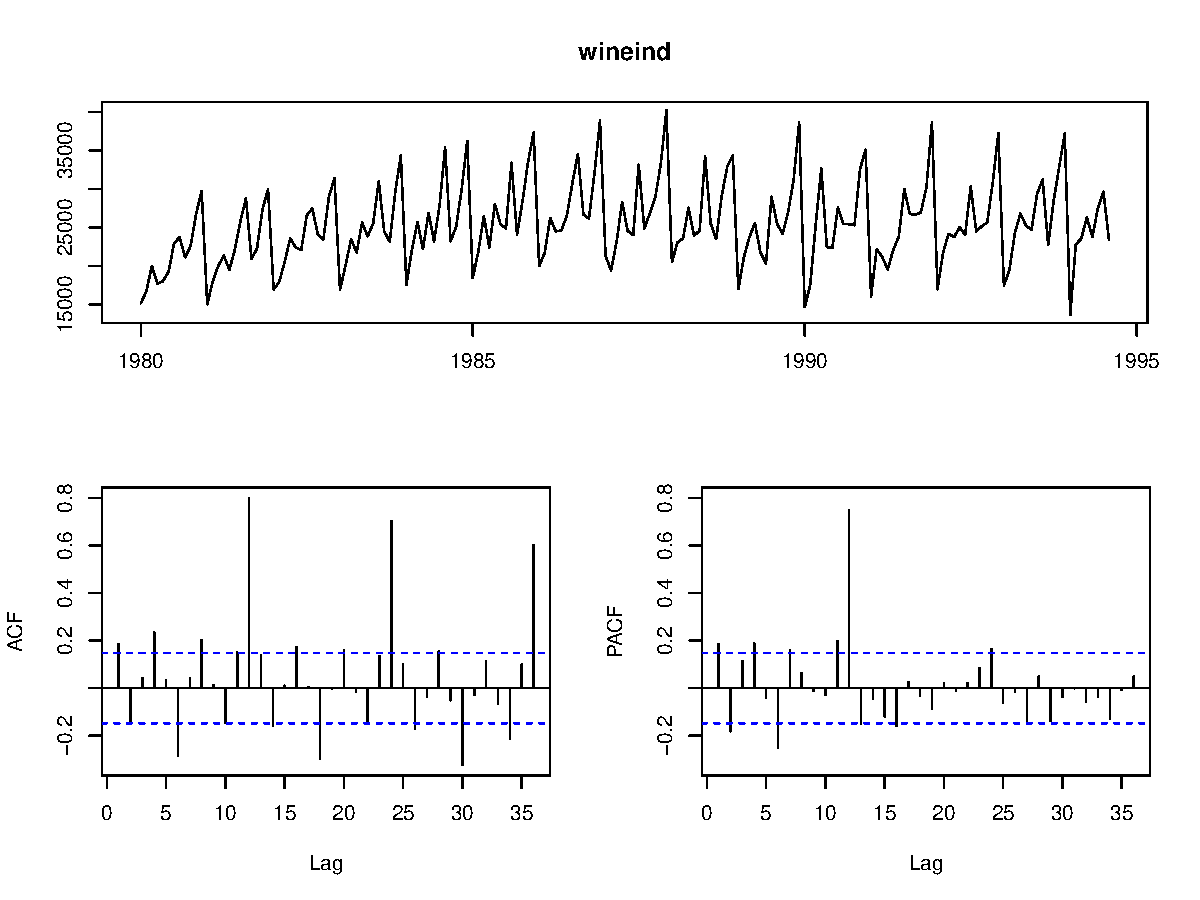
\includegraphics{Lec11_files/figure-beamer/unnamed-chunk-1-1.pdf}

\end{frame}

\begin{frame}{Differencing}

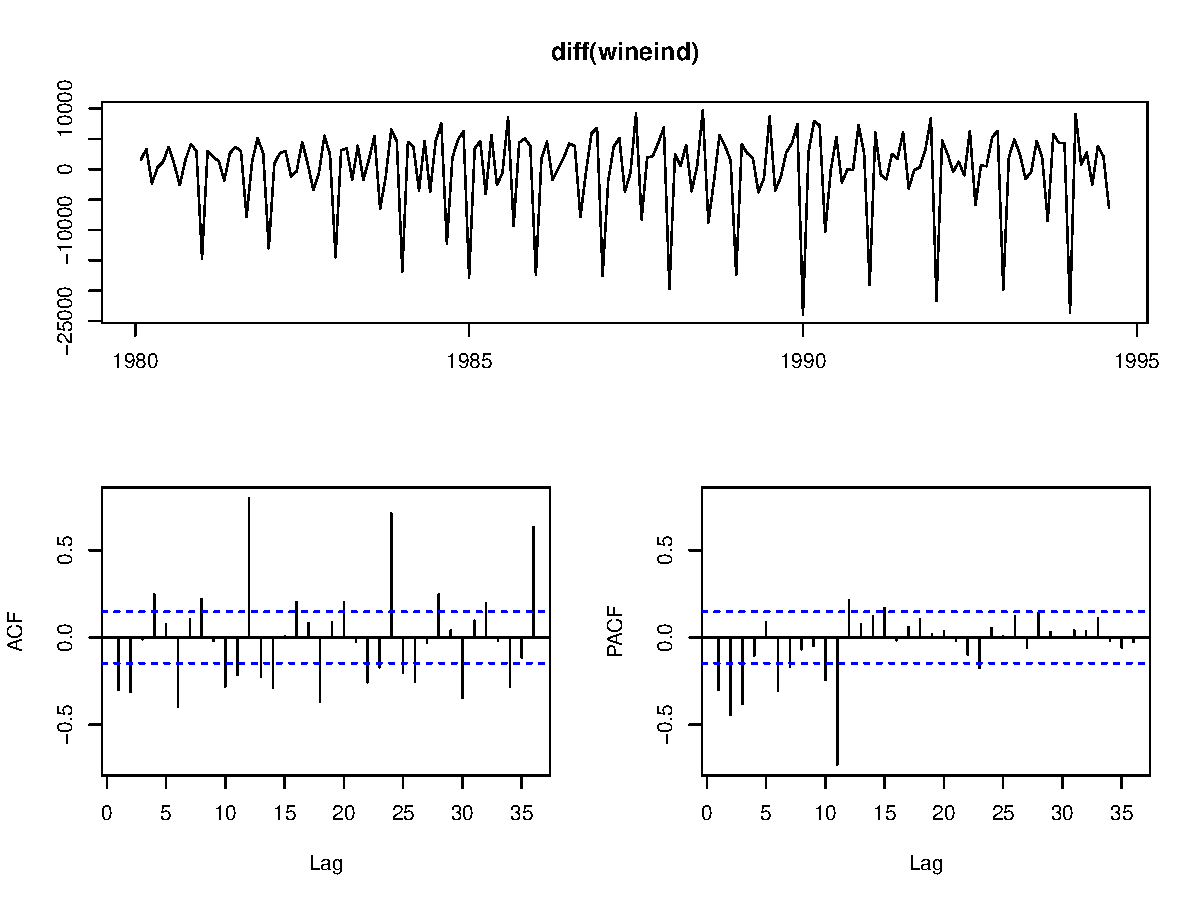
\includegraphics{Lec11_files/figure-beamer/unnamed-chunk-2-1.pdf}

\end{frame}

\begin{frame}[t]{Seasonal ARIMA}

We can extend the existing ARIMA model to handle these higher order lags
(without having to include all of the intervening lags).

\vspace{3mm}

Seasonal \(\text{ARIMA}\,(p,d,q) \times (P,D,Q)_s\):
\[ \Phi_P(L^s) \, \phi_p(L) \, \Delta_s^D \, \Delta^d \, y_t = \delta + \Theta_Q(L^s) \, \theta_q(L) \, w_t\]
\pause where \[
\begin{aligned}
\phi_p(L) &= 1-\phi_1 L - \phi_2 L^2 - \ldots - \phi_p L^p\\
\theta_q(L) &= 1+\theta_1 L + \theta_2 L^2 + \ldots + \theta_p L^q \\
\Delta^d &= (1-L)^d\\
\\
\Phi_P(L^s) &= 1-\Phi_1 L^s - \Phi_2 L^{2s} - \ldots - \Phi_P L^{Ps} \\
\Theta_Q(L^s) &= 1+\Theta_1 L + \Theta_2 L^{2s} + \ldots + \theta_p L^{Qs} \\
\Delta_s^D &= (1-L^s)^D\\
\end{aligned}
\]

\end{frame}

\begin{frame}[fragile]{Seasonal ARIMA for \texttt{wineind}}

Lets consider an \(\text{ARIMA}(0,0,0) \times (1,0,0)_{12}\): \[
\begin{aligned}
(1-\Phi_1 L^{12}) \, y_t = \delta + w_t \\
y_t = \Phi_1 y_{t-12} + \delta + w_t
\end{aligned}
\] \vspace{2mm}

\begin{Shaded}
\begin{Highlighting}[]
\NormalTok{(}\DataTypeTok{m1 =} \KeywordTok{Arima}\NormalTok{(wineind, }\DataTypeTok{seasonal=}\KeywordTok{list}\NormalTok{(}\DataTypeTok{order=}\KeywordTok{c}\NormalTok{(}\DecValTok{1}\NormalTok{,}\DecValTok{0}\NormalTok{,}\DecValTok{0}\NormalTok{), }\DataTypeTok{period=}\DecValTok{12}\NormalTok{)))}
\NormalTok{## Series: wineind }
\NormalTok{## ARIMA(0,0,0)(1,0,0)[12] with non-zero mean }
\NormalTok{## }
\NormalTok{## Coefficients:}
\NormalTok{##         sar1       mean}
\NormalTok{##       0.8780  24489.243}
\NormalTok{## s.e.  0.0314   1154.487}
\NormalTok{## }
\NormalTok{## sigma^2 estimated as 6906536:  log likelihood=-1643.39}
\NormalTok{## AIC=3292.78   AICc=3292.92   BIC=3302.29}
\end{Highlighting}
\end{Shaded}

\end{frame}

\begin{frame}{Fitted model}

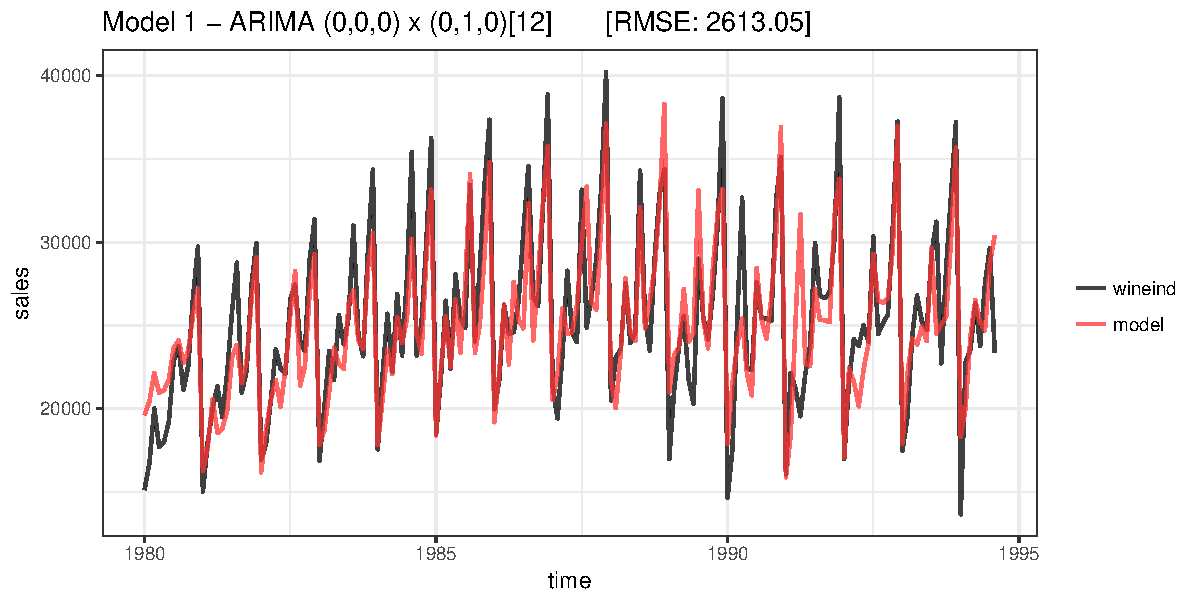
\includegraphics{Lec11_files/figure-beamer/unnamed-chunk-4-1.pdf}

\end{frame}

\begin{frame}{Residuals}

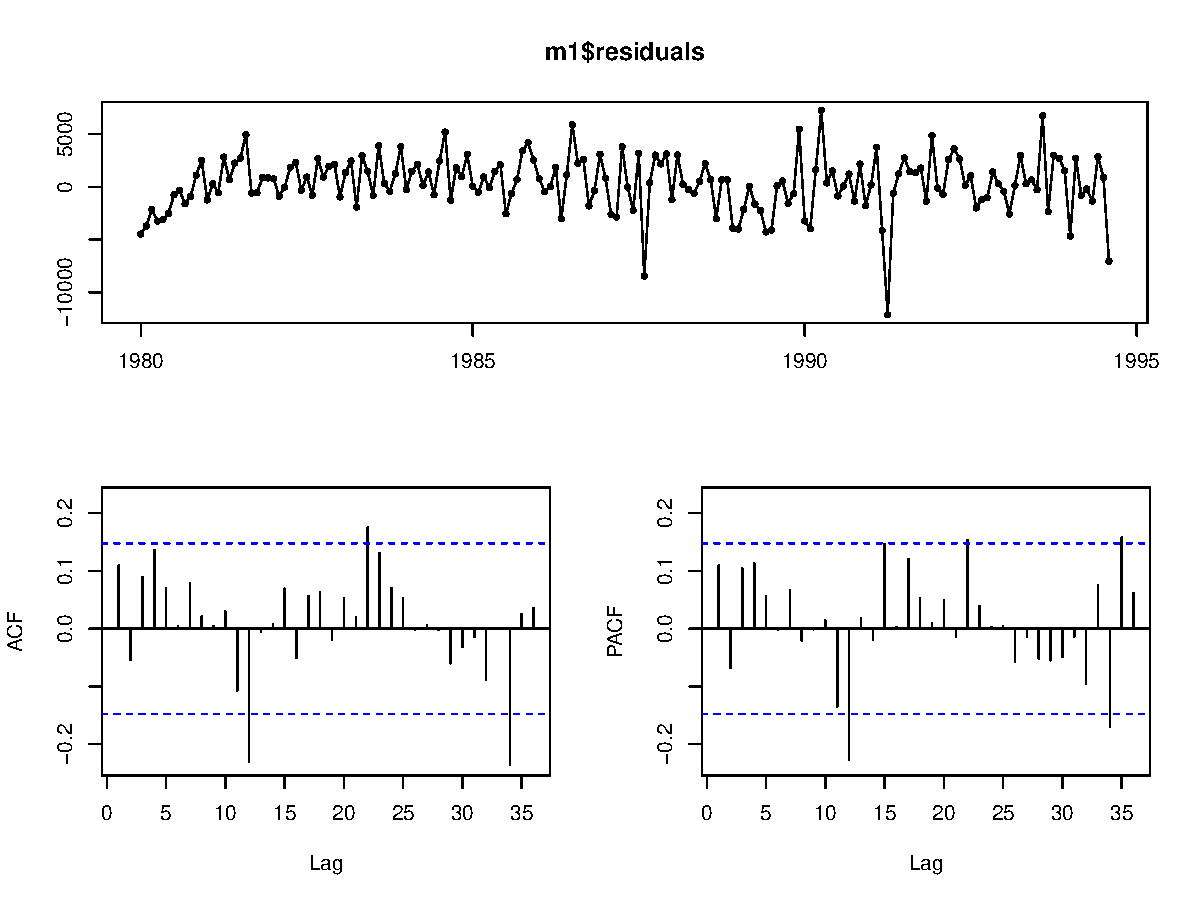
\includegraphics{Lec11_files/figure-beamer/unnamed-chunk-5-1.pdf}

\end{frame}

\begin{frame}[fragile]{Model 2}

\(\text{ARIMA}(0,0,0) \times (0,1,1)_{12}\): \[
\begin{aligned}
(1-L^{12}) y_t = \delta + (1+\Theta_1 L^{12})  w_t \\
y_t-y_{t-12} = \delta + w_t + \Theta_1 w_{t-12} \\
y_t = \delta + y_{t-12} + w_t + \Theta_1 w_{t-12}
\end{aligned}
\]

\begin{Shaded}
\begin{Highlighting}[]
\NormalTok{(}\DataTypeTok{m2 =} \KeywordTok{Arima}\NormalTok{(wineind, }\DataTypeTok{order=}\KeywordTok{c}\NormalTok{(}\DecValTok{0}\NormalTok{,}\DecValTok{0}\NormalTok{,}\DecValTok{0}\NormalTok{), }\DataTypeTok{seasonal=}\KeywordTok{list}\NormalTok{(}\DataTypeTok{order=}\KeywordTok{c}\NormalTok{(}\DecValTok{0}\NormalTok{,}\DecValTok{1}\NormalTok{,}\DecValTok{1}\NormalTok{), }\DataTypeTok{period=}\DecValTok{12}\NormalTok{)))}
\NormalTok{## Series: wineind }
\NormalTok{## ARIMA(0,0,0)(0,1,1)[12]                    }
\NormalTok{## }
\NormalTok{## Coefficients:}
\NormalTok{##          sma1}
\NormalTok{##       -0.3246}
\NormalTok{## s.e.   0.0807}
\NormalTok{## }
\NormalTok{## sigma^2 estimated as 6588531:  log likelihood=-1520.34}
\NormalTok{## AIC=3044.68   AICc=3044.76   BIC=3050.88}
\end{Highlighting}
\end{Shaded}

\end{frame}

\begin{frame}{Fitted model}

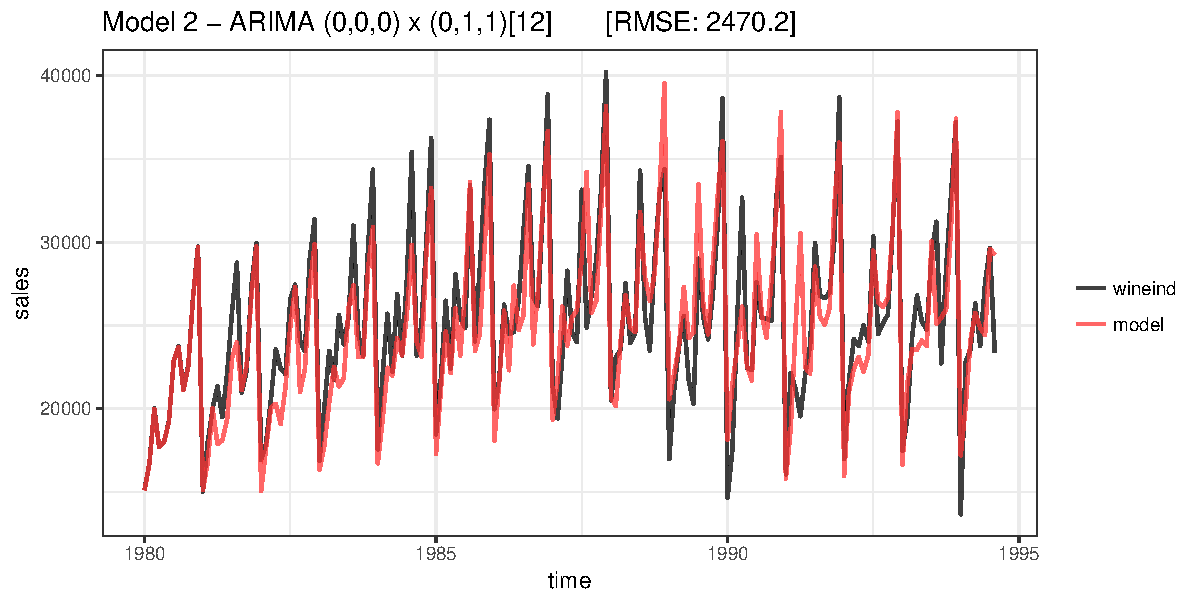
\includegraphics{Lec11_files/figure-beamer/unnamed-chunk-7-1.pdf}

\end{frame}

\begin{frame}{Residuals}

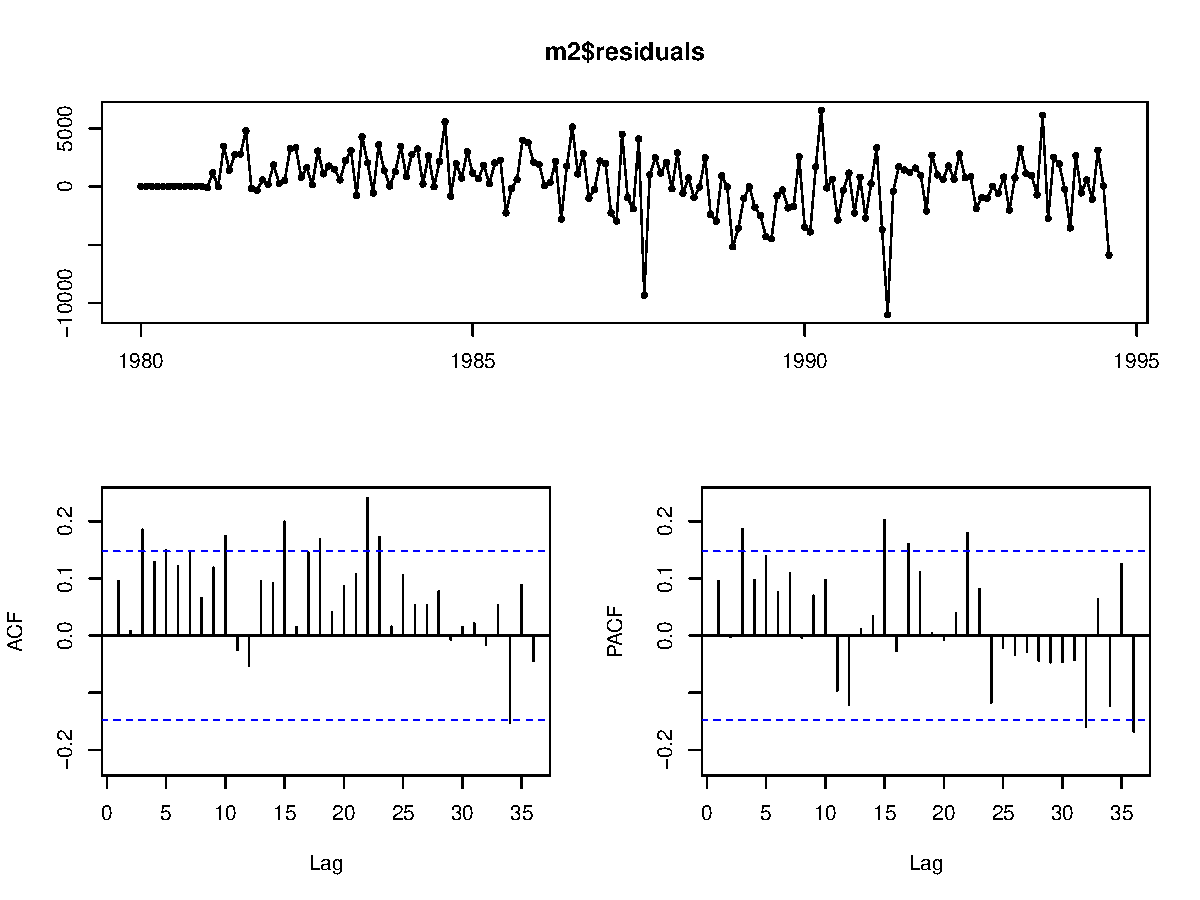
\includegraphics{Lec11_files/figure-beamer/unnamed-chunk-8-1.pdf}

\end{frame}

\begin{frame}[fragile]{Model 3}

\(\text{ARIMA}(3,0,0) \times (0,1,1)_{12}\) \[
\begin{aligned}
(1-\phi_1 L - \phi_2 L^2 - \phi_3 L^3) \, (1-L^{12}) y_t = \delta + (1 + \Theta_1 L)w_t \\
(1-\phi_1 L - \phi_2 L^2 - \phi_3 L^3) \, (y_t-y_{t-12}) = \delta + w_t + w_{t-12} \\
y_t = \delta + \sum_{i=1}^3 \phi_i y_{t-1}  + y_{t-12}  - \sum_{i=1}^3 \phi_i y_{t-12-i} + w_t + w_{t-12}
\end{aligned}
\]

\begin{Shaded}
\begin{Highlighting}[]
\NormalTok{(}\DataTypeTok{m3 =} \KeywordTok{Arima}\NormalTok{(wineind, }\DataTypeTok{order=}\KeywordTok{c}\NormalTok{(}\DecValTok{3}\NormalTok{,}\DecValTok{0}\NormalTok{,}\DecValTok{0}\NormalTok{), }
            \DataTypeTok{seasonal=}\KeywordTok{list}\NormalTok{(}\DataTypeTok{order=}\KeywordTok{c}\NormalTok{(}\DecValTok{0}\NormalTok{,}\DecValTok{1}\NormalTok{,}\DecValTok{1}\NormalTok{), }\DataTypeTok{period=}\DecValTok{12}\NormalTok{)))}
\NormalTok{## Series: wineind }
\NormalTok{## ARIMA(3,0,0)(0,1,1)[12]                    }
\NormalTok{## }
\NormalTok{## Coefficients:}
\NormalTok{##          ar1     ar2     ar3     sma1}
\NormalTok{##       0.1402  0.0806  0.3040  -0.5790}
\NormalTok{## s.e.  0.0755  0.0813  0.0823   0.1023}
\NormalTok{## }
\NormalTok{## sigma^2 estimated as 5948935:  log likelihood=-1512.38}
\NormalTok{## AIC=3034.77   AICc=3035.15   BIC=3050.27}
\end{Highlighting}
\end{Shaded}

\end{frame}

\begin{frame}{Fitted model}

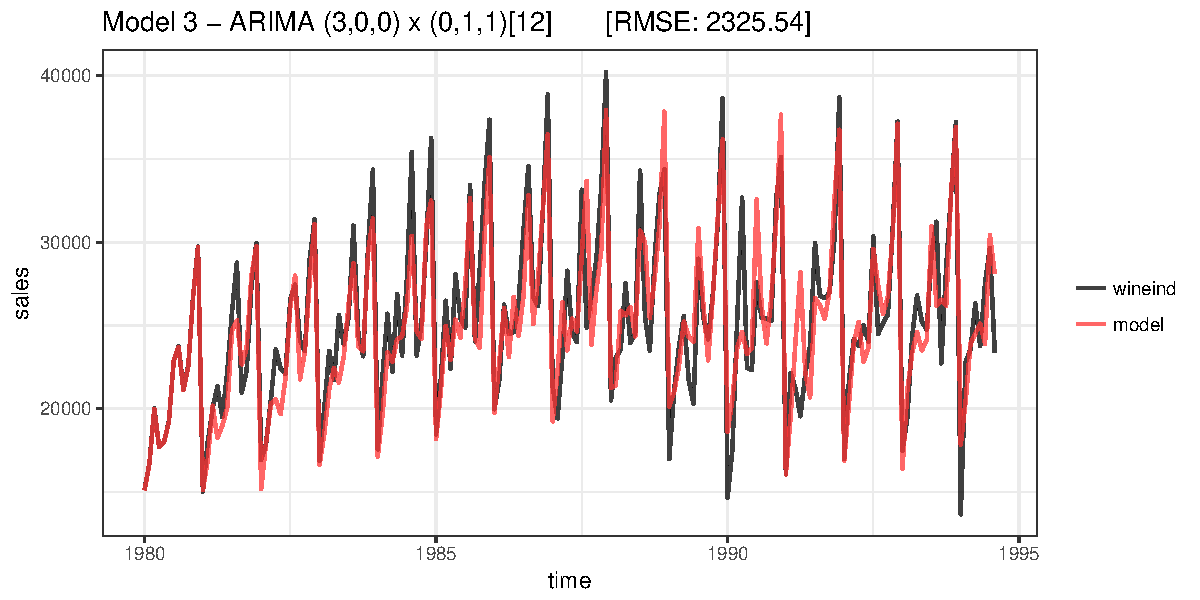
\includegraphics{Lec11_files/figure-beamer/unnamed-chunk-10-1.pdf}

\end{frame}

\begin{frame}{Model - Residuals}

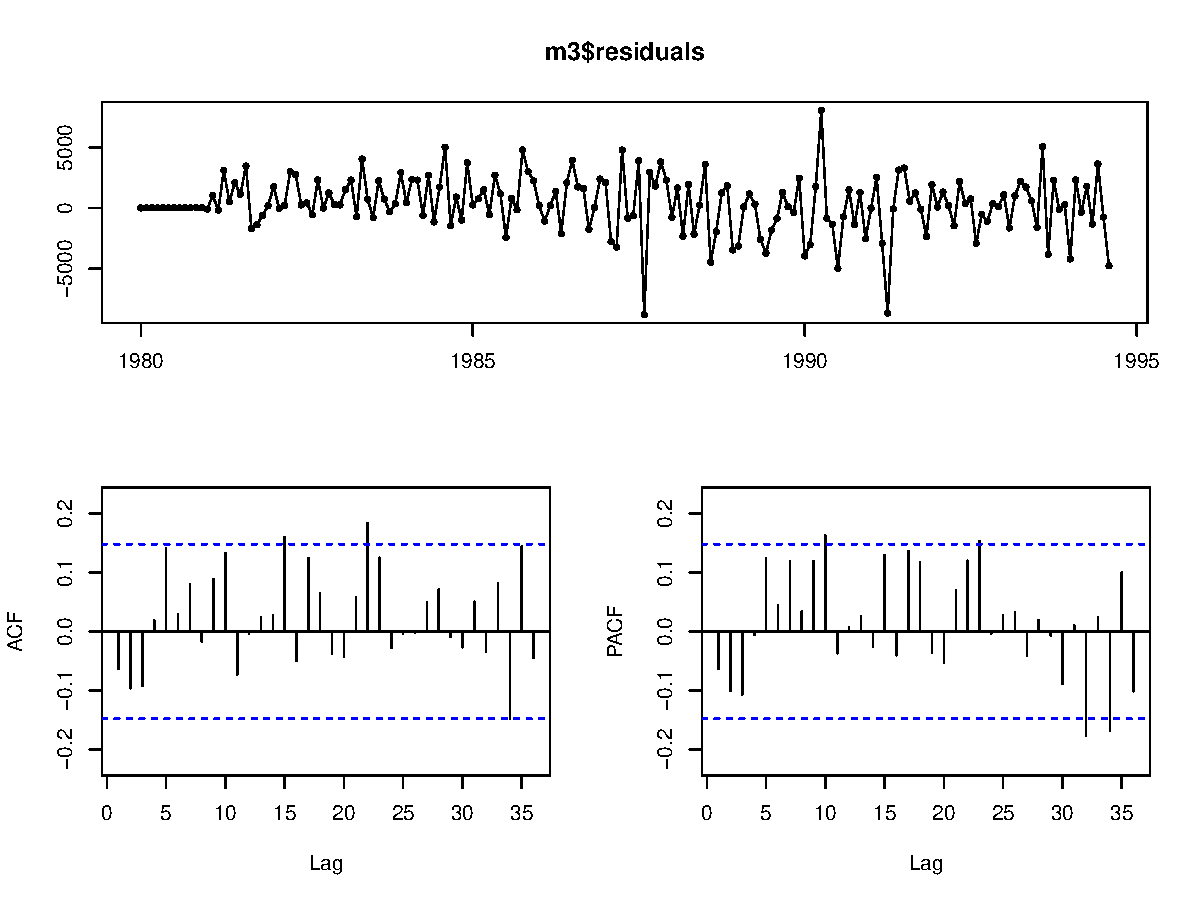
\includegraphics{Lec11_files/figure-beamer/unnamed-chunk-11-1.pdf}

\end{frame}

\section{Federal Reserve Board Production
Index}\label{federal-reserve-board-production-index}

\begin{frame}{\texttt{prodn} from the \texttt{astsa} package}

Monthly Federal Reserve Board Production Index (1948-1978)

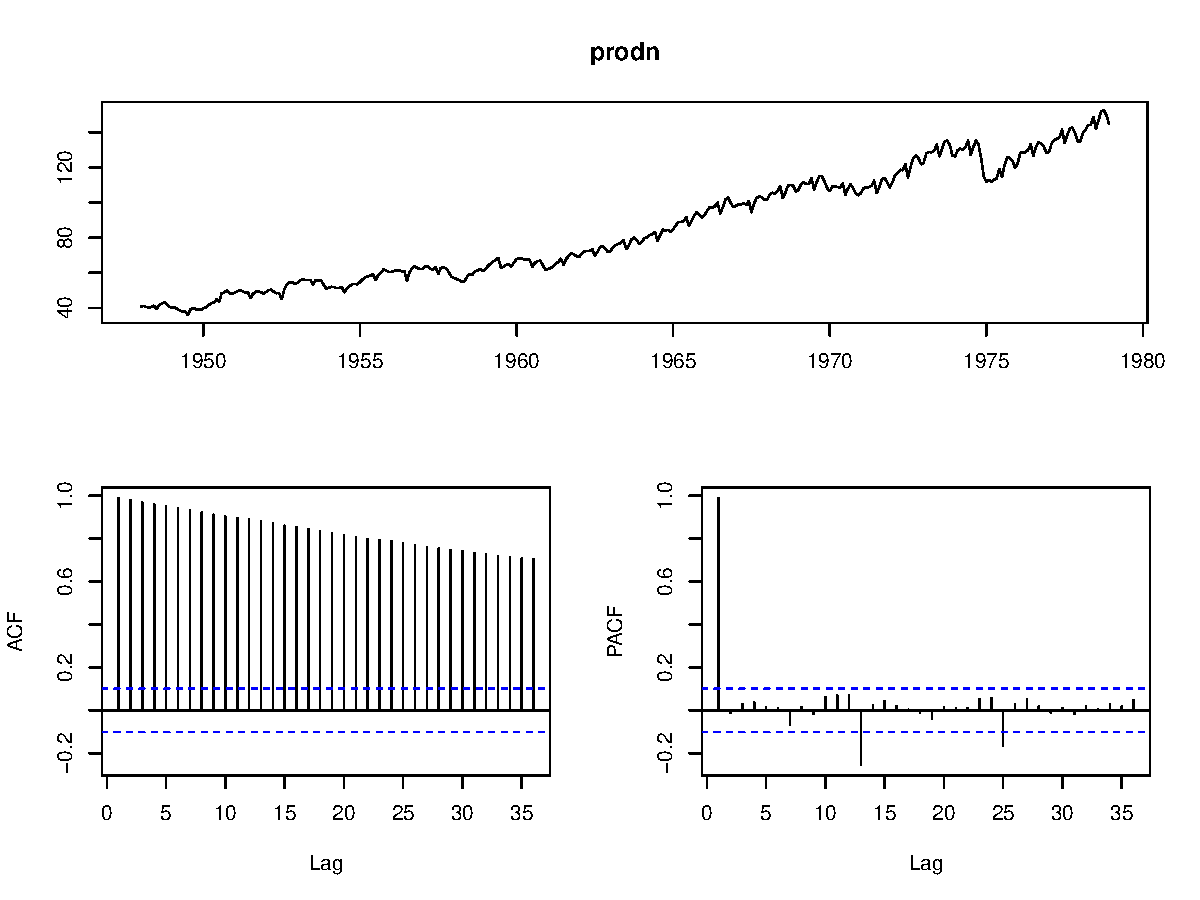
\includegraphics{Lec11_files/figure-beamer/unnamed-chunk-12-1.pdf}

\end{frame}

\begin{frame}{Differencing}

Based on the ACF it seems like standard differencing may be required

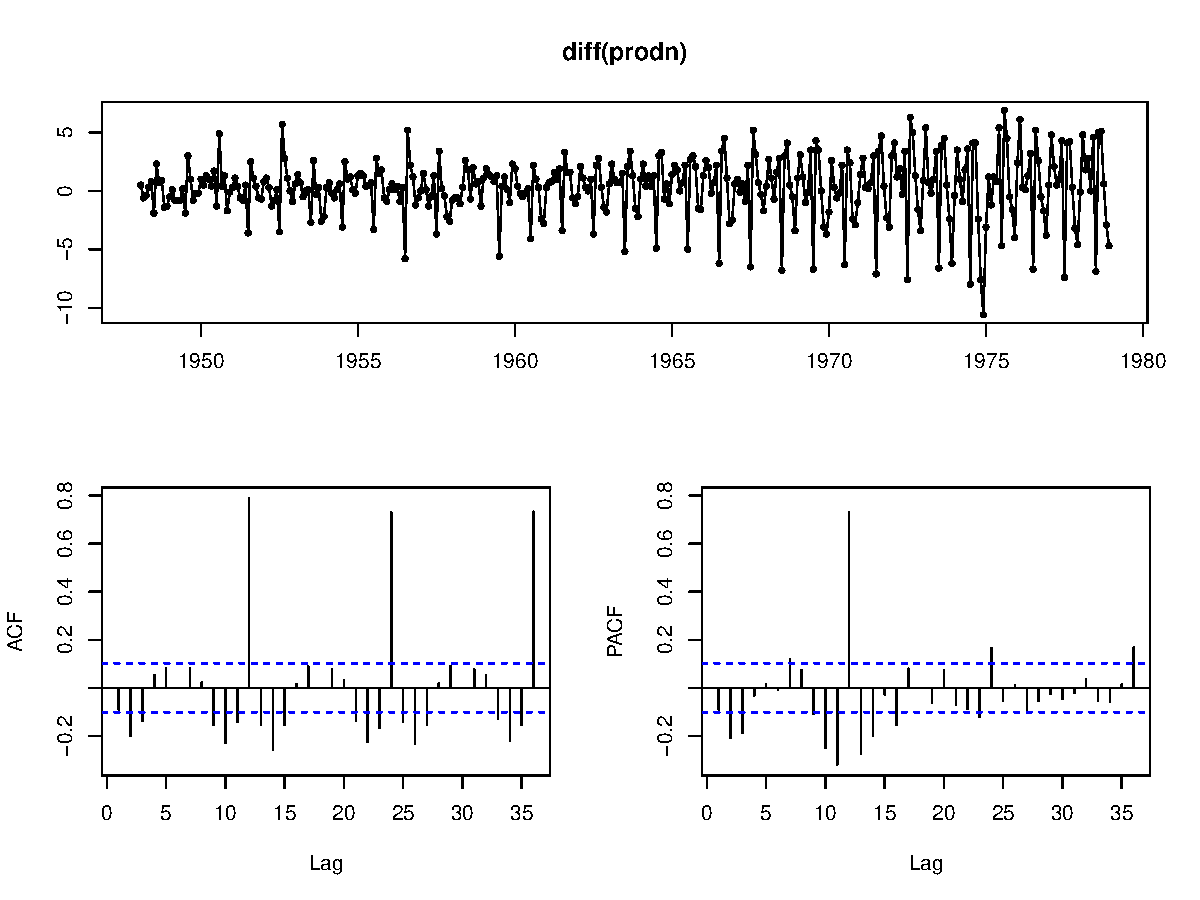
\includegraphics{Lec11_files/figure-beamer/unnamed-chunk-13-1.pdf}

\end{frame}

\begin{frame}[fragile]{Differencing + Seasonal Differencing}

Additional seasonal differencing also seems warranted

\begin{Shaded}
\begin{Highlighting}[]
\NormalTok{(}\DataTypeTok{fr_m1 =} \KeywordTok{Arima}\NormalTok{(prodn, }\DataTypeTok{order =} \KeywordTok{c}\NormalTok{(}\DecValTok{0}\NormalTok{,}\DecValTok{1}\NormalTok{,}\DecValTok{0}\NormalTok{), }
            \DataTypeTok{seasonal =} \KeywordTok{list}\NormalTok{(}\DataTypeTok{order=}\KeywordTok{c}\NormalTok{(}\DecValTok{0}\NormalTok{,}\DecValTok{0}\NormalTok{,}\DecValTok{0}\NormalTok{), }\DataTypeTok{period=}\DecValTok{12}\NormalTok{)))}
\NormalTok{## Series: prodn }
\NormalTok{## ARIMA(0,1,0)                    }
\NormalTok{## }
\NormalTok{## sigma^2 estimated as 7.147:  log likelihood=-891.26}
\NormalTok{## AIC=1784.51   AICc=1784.52   BIC=1788.43}
\end{Highlighting}
\end{Shaded}

\begin{Shaded}
\begin{Highlighting}[]
\NormalTok{(}\DataTypeTok{fr_m2 =} \KeywordTok{Arima}\NormalTok{(prodn, }\DataTypeTok{order =} \KeywordTok{c}\NormalTok{(}\DecValTok{0}\NormalTok{,}\DecValTok{1}\NormalTok{,}\DecValTok{0}\NormalTok{), }
            \DataTypeTok{seasonal =} \KeywordTok{list}\NormalTok{(}\DataTypeTok{order=}\KeywordTok{c}\NormalTok{(}\DecValTok{0}\NormalTok{,}\DecValTok{1}\NormalTok{,}\DecValTok{0}\NormalTok{), }\DataTypeTok{period=}\DecValTok{12}\NormalTok{)))}
\NormalTok{## Series: prodn }
\NormalTok{## ARIMA(0,1,0)(0,1,0)[12]                    }
\NormalTok{## }
\NormalTok{## sigma^2 estimated as 2.52:  log likelihood=-675.29}
\NormalTok{## AIC=1352.58   AICc=1352.59   BIC=1356.46}
\end{Highlighting}
\end{Shaded}

\end{frame}

\begin{frame}{Residuals}

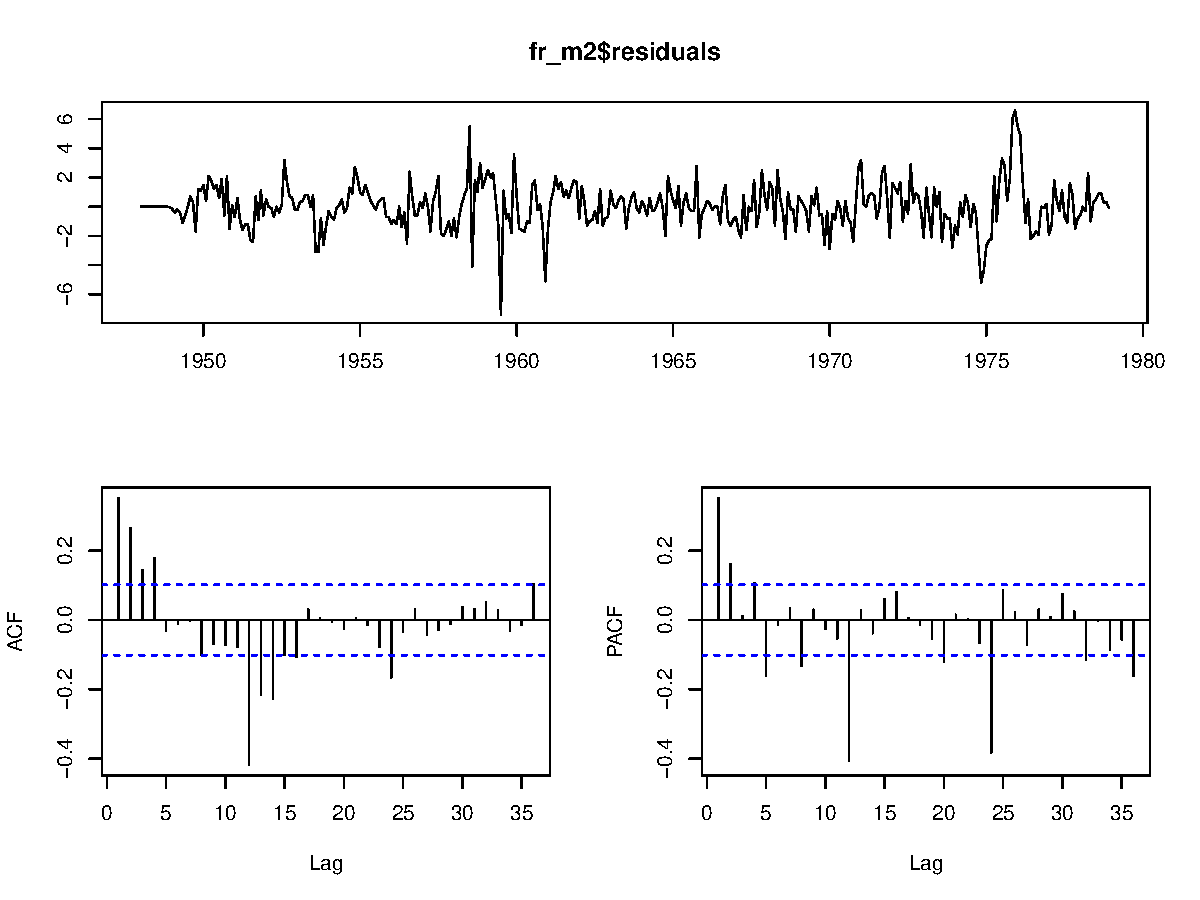
\includegraphics{Lec11_files/figure-beamer/unnamed-chunk-16-1.pdf}

\end{frame}

\begin{frame}[fragile]{Adding Seasonal MA}

\scriptoutput

\begin{Shaded}
\begin{Highlighting}[]
\NormalTok{(}\DataTypeTok{fr_m3.1 =} \KeywordTok{Arima}\NormalTok{(prodn, }\DataTypeTok{order =} \KeywordTok{c}\NormalTok{(}\DecValTok{0}\NormalTok{,}\DecValTok{1}\NormalTok{,}\DecValTok{0}\NormalTok{), }
            \DataTypeTok{seasonal =} \KeywordTok{list}\NormalTok{(}\DataTypeTok{order=}\KeywordTok{c}\NormalTok{(}\DecValTok{0}\NormalTok{,}\DecValTok{1}\NormalTok{,}\DecValTok{1}\NormalTok{), }\DataTypeTok{period=}\DecValTok{12}\NormalTok{)))}
\NormalTok{## Series: prodn }
\NormalTok{## ARIMA(0,1,0)(0,1,1)[12]                    }
\NormalTok{## }
\NormalTok{## Coefficients:}
\NormalTok{##          sma1}
\NormalTok{##       -0.7151}
\NormalTok{## s.e.   0.0317}
\NormalTok{## }
\NormalTok{## sigma^2 estimated as 1.616:  log likelihood=-599.29}
\NormalTok{## AIC=1202.57   AICc=1202.61   BIC=1210.34}
\end{Highlighting}
\end{Shaded}

\begin{Shaded}
\begin{Highlighting}[]
\NormalTok{(}\DataTypeTok{fr_m3.2 =} \KeywordTok{Arima}\NormalTok{(prodn, }\DataTypeTok{order =} \KeywordTok{c}\NormalTok{(}\DecValTok{0}\NormalTok{,}\DecValTok{1}\NormalTok{,}\DecValTok{0}\NormalTok{), }
            \DataTypeTok{seasonal =} \KeywordTok{list}\NormalTok{(}\DataTypeTok{order=}\KeywordTok{c}\NormalTok{(}\DecValTok{0}\NormalTok{,}\DecValTok{1}\NormalTok{,}\DecValTok{2}\NormalTok{), }\DataTypeTok{period=}\DecValTok{12}\NormalTok{)))}
\NormalTok{## Series: prodn }
\NormalTok{## ARIMA(0,1,0)(0,1,2)[12]                    }
\NormalTok{## }
\NormalTok{## Coefficients:}
\NormalTok{##          sma1    sma2}
\NormalTok{##       -0.7624  0.0520}
\NormalTok{## s.e.   0.0689  0.0666}
\NormalTok{## }
\NormalTok{## sigma^2 estimated as 1.615:  log likelihood=-598.98}
\NormalTok{## AIC=1203.96   AICc=1204.02   BIC=1215.61}
\end{Highlighting}
\end{Shaded}

\end{frame}

\begin{frame}[fragile,t]{Adding Seasonal MA (cont.)}

\scriptoutput 

\begin{Shaded}
\begin{Highlighting}[]
\NormalTok{(}\DataTypeTok{fr_m3.3 =} \KeywordTok{Arima}\NormalTok{(prodn, }\DataTypeTok{order =} \KeywordTok{c}\NormalTok{(}\DecValTok{0}\NormalTok{,}\DecValTok{1}\NormalTok{,}\DecValTok{0}\NormalTok{), }
            \DataTypeTok{seasonal =} \KeywordTok{list}\NormalTok{(}\DataTypeTok{order=}\KeywordTok{c}\NormalTok{(}\DecValTok{0}\NormalTok{,}\DecValTok{1}\NormalTok{,}\DecValTok{3}\NormalTok{), }\DataTypeTok{period=}\DecValTok{12}\NormalTok{)))}
\NormalTok{## Series: prodn }
\NormalTok{## ARIMA(0,1,0)(0,1,3)[12]                    }
\NormalTok{## }
\NormalTok{## Coefficients:}
\NormalTok{##          sma1     sma2    sma3}
\NormalTok{##       -0.7853  -0.1205  0.2624}
\NormalTok{## s.e.   0.0529   0.0644  0.0529}
\NormalTok{## }
\NormalTok{## sigma^2 estimated as 1.506:  log likelihood=-587.58}
\NormalTok{## AIC=1183.15   AICc=1183.27   BIC=1198.69}
\end{Highlighting}
\end{Shaded}

\end{frame}

\begin{frame}{Residuals - Model 3.3}

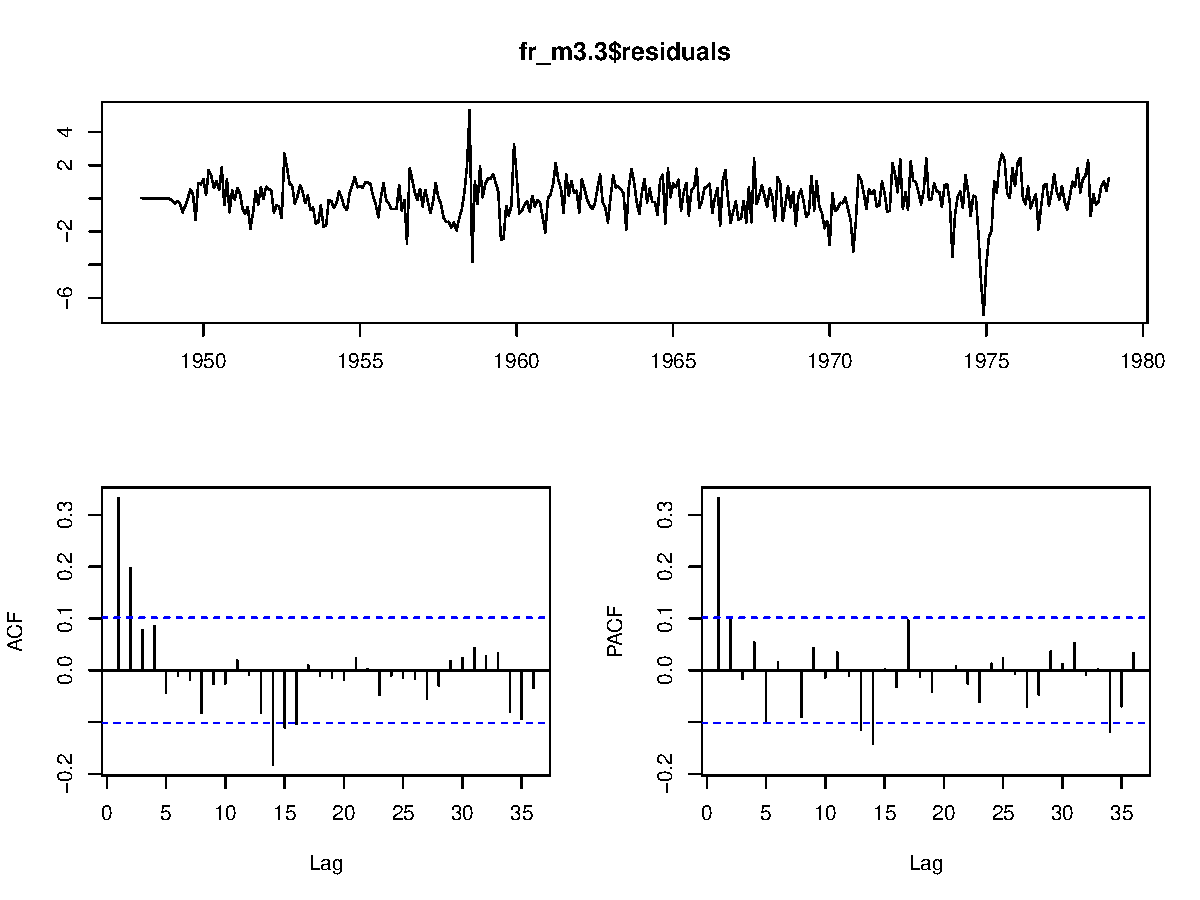
\includegraphics{Lec11_files/figure-beamer/unnamed-chunk-20-1.pdf}

\end{frame}

\begin{frame}[fragile]{Adding AR}

\scriptoutput

\begin{Shaded}
\begin{Highlighting}[]
\NormalTok{(}\DataTypeTok{fr_m4.1 =} \KeywordTok{Arima}\NormalTok{(prodn, }\DataTypeTok{order =} \KeywordTok{c}\NormalTok{(}\DecValTok{1}\NormalTok{,}\DecValTok{1}\NormalTok{,}\DecValTok{0}\NormalTok{), }
            \DataTypeTok{seasonal =} \KeywordTok{list}\NormalTok{(}\DataTypeTok{order=}\KeywordTok{c}\NormalTok{(}\DecValTok{0}\NormalTok{,}\DecValTok{1}\NormalTok{,}\DecValTok{3}\NormalTok{), }\DataTypeTok{period=}\DecValTok{12}\NormalTok{)))}
\NormalTok{## Series: prodn }
\NormalTok{## ARIMA(1,1,0)(0,1,3)[12]                    }
\NormalTok{## }
\NormalTok{## Coefficients:}
\NormalTok{##          ar1     sma1     sma2    sma3}
\NormalTok{##       0.3393  -0.7619  -0.1222  0.2756}
\NormalTok{## s.e.  0.0500   0.0527   0.0646  0.0525}
\NormalTok{## }
\NormalTok{## sigma^2 estimated as 1.341:  log likelihood=-565.98}
\NormalTok{## AIC=1141.95   AICc=1142.12   BIC=1161.37}
\end{Highlighting}
\end{Shaded}

\begin{Shaded}
\begin{Highlighting}[]
\NormalTok{(}\DataTypeTok{fr_m4.2 =} \KeywordTok{Arima}\NormalTok{(prodn, }\DataTypeTok{order =} \KeywordTok{c}\NormalTok{(}\DecValTok{2}\NormalTok{,}\DecValTok{1}\NormalTok{,}\DecValTok{0}\NormalTok{), }
            \DataTypeTok{seasonal =} \KeywordTok{list}\NormalTok{(}\DataTypeTok{order=}\KeywordTok{c}\NormalTok{(}\DecValTok{0}\NormalTok{,}\DecValTok{1}\NormalTok{,}\DecValTok{3}\NormalTok{), }\DataTypeTok{period=}\DecValTok{12}\NormalTok{)))}
\NormalTok{## Series: prodn }
\NormalTok{## ARIMA(2,1,0)(0,1,3)[12]                    }
\NormalTok{## }
\NormalTok{## Coefficients:}
\NormalTok{##          ar1     ar2     sma1     sma2    sma3}
\NormalTok{##       0.3038  0.1077  -0.7393  -0.1445  0.2815}
\NormalTok{## s.e.  0.0526  0.0538   0.0539   0.0653  0.0526}
\NormalTok{## }
\NormalTok{## sigma^2 estimated as 1.331:  log likelihood=-563.98}
\NormalTok{## AIC=1139.97   AICc=1140.2   BIC=1163.26}
\end{Highlighting}
\end{Shaded}

\end{frame}

\begin{frame}{Residuals - Model 4.1}

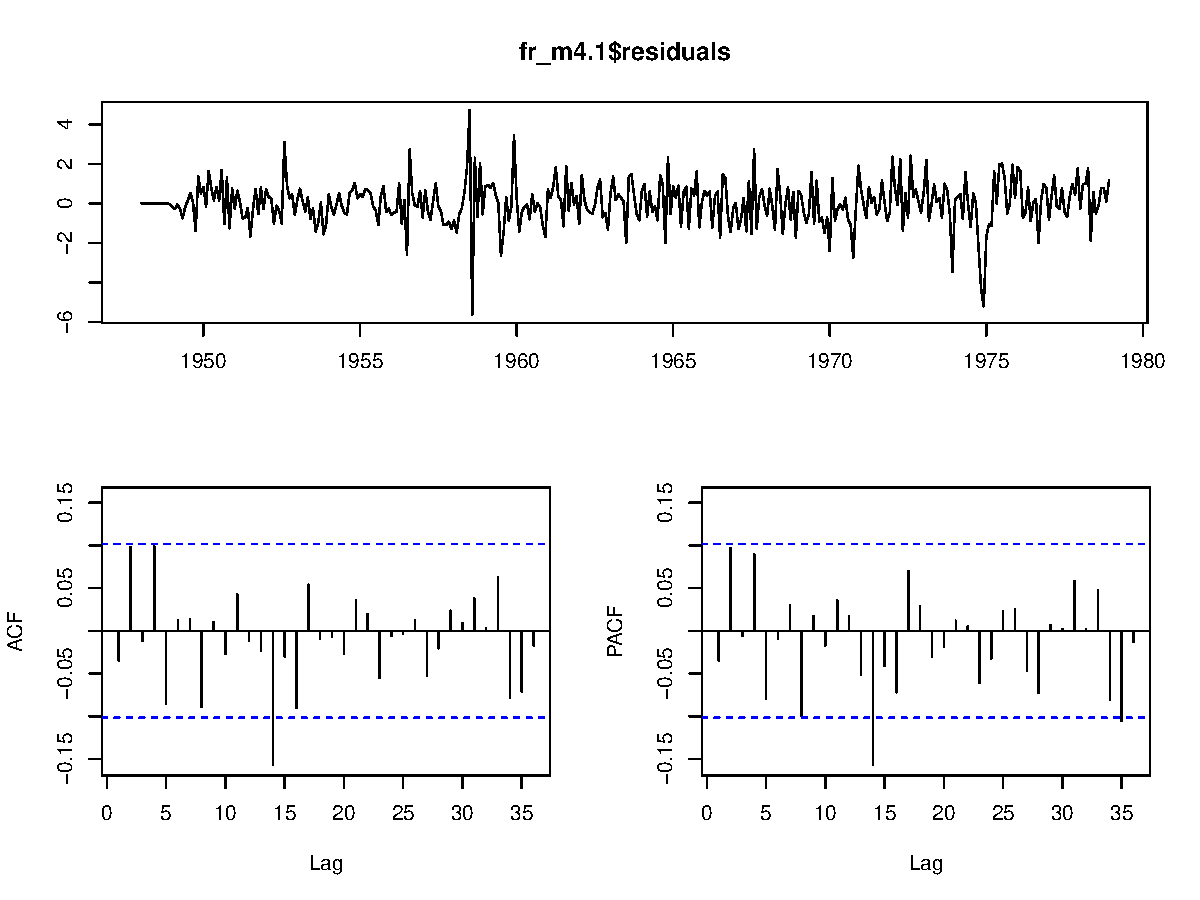
\includegraphics{Lec11_files/figure-beamer/unnamed-chunk-23-1.pdf}

\end{frame}

\begin{frame}{Residuals - Model 4.2}

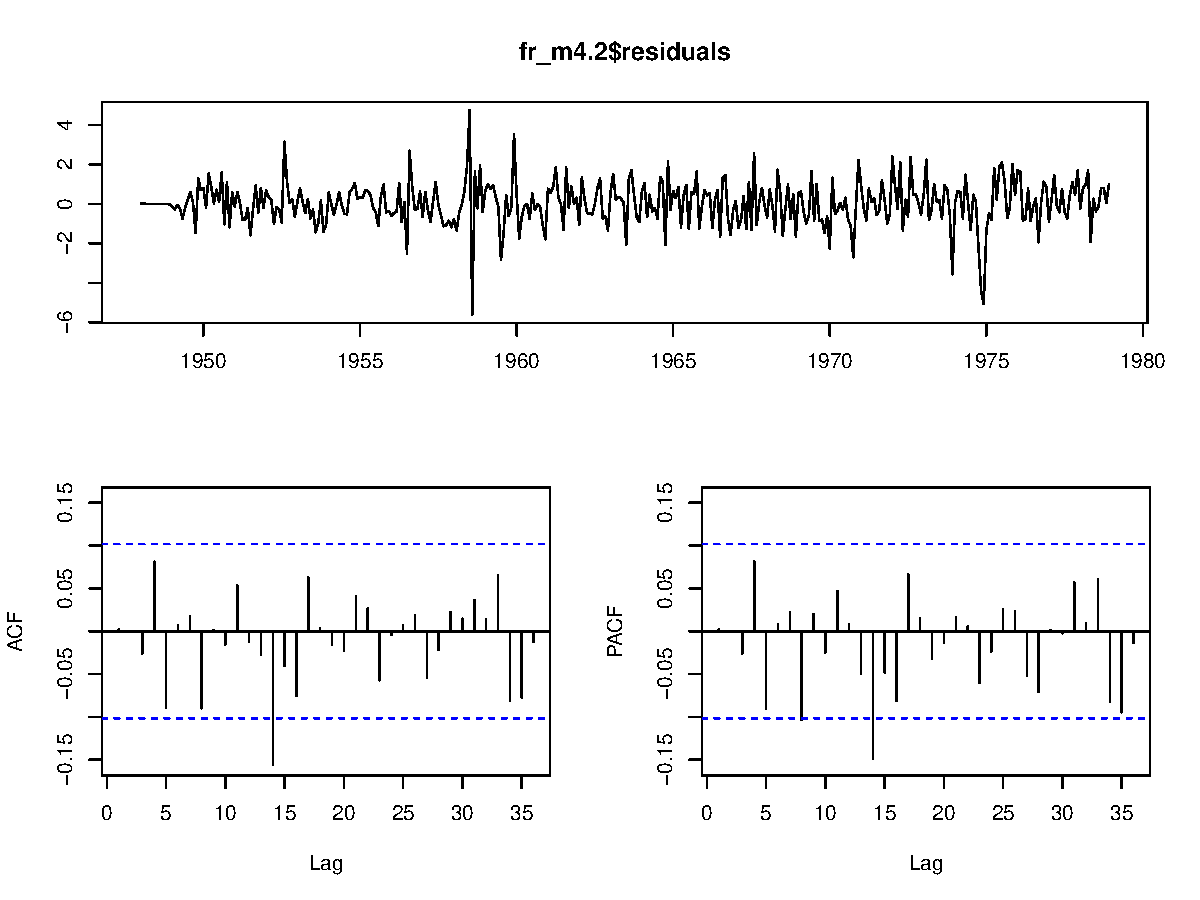
\includegraphics{Lec11_files/figure-beamer/unnamed-chunk-24-1.pdf}

\end{frame}

\begin{frame}{Model Fit}

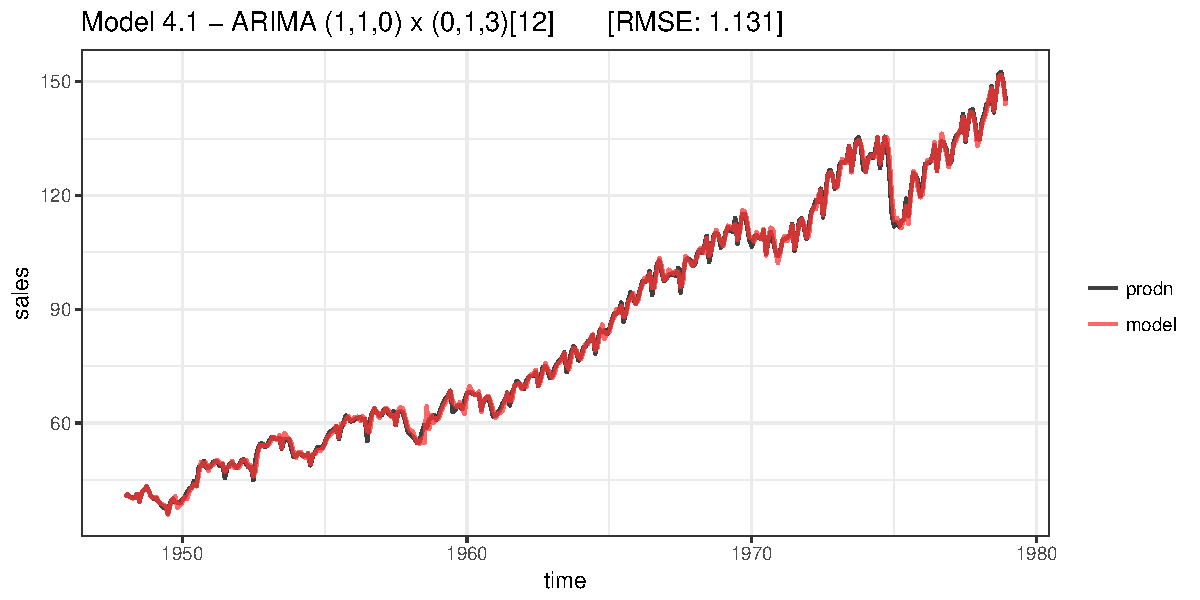
\includegraphics{Lec11_files/figure-beamer/unnamed-chunk-25-1.pdf}

\end{frame}

\begin{frame}{Model Forecast}

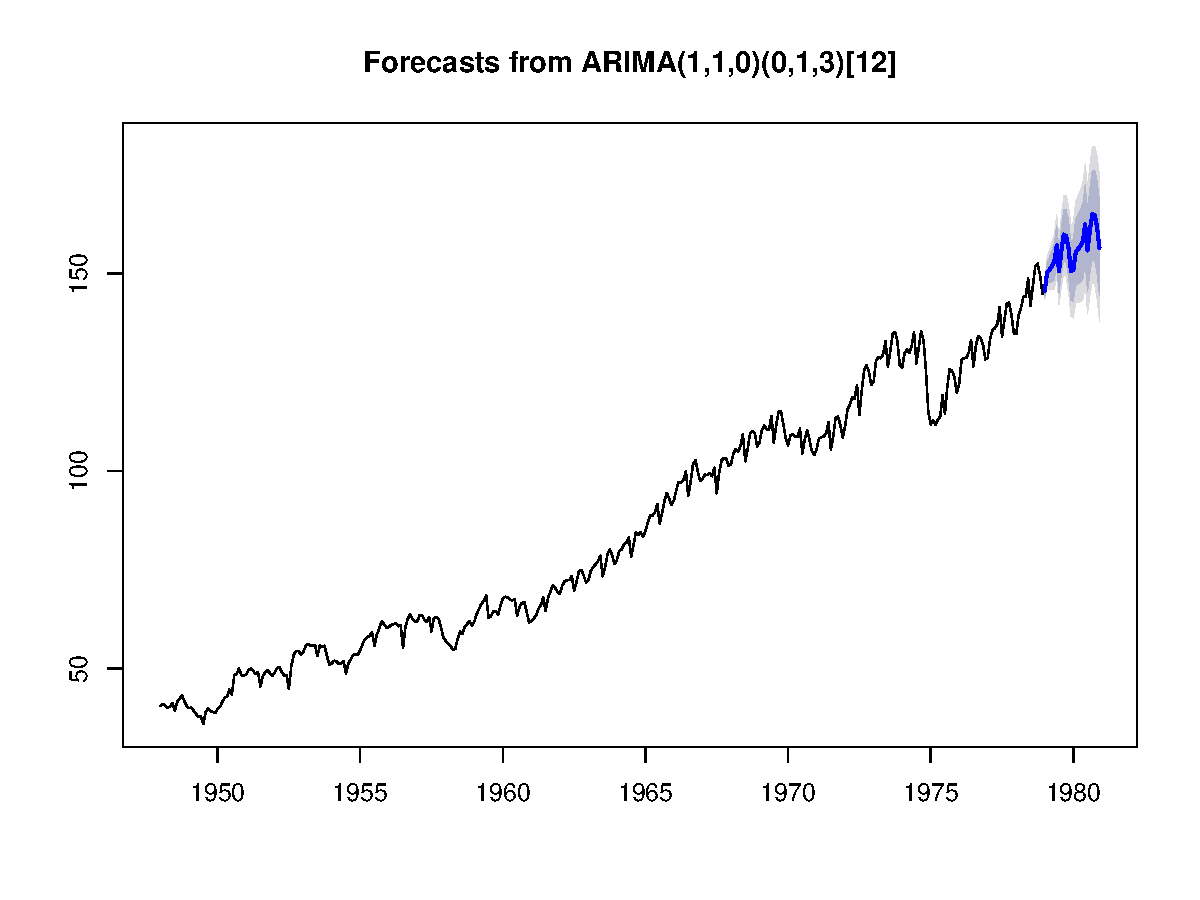
\includegraphics{Lec11_files/figure-beamer/unnamed-chunk-26-1.pdf}

\end{frame}

\begin{frame}{Model Forecast (cont.)}

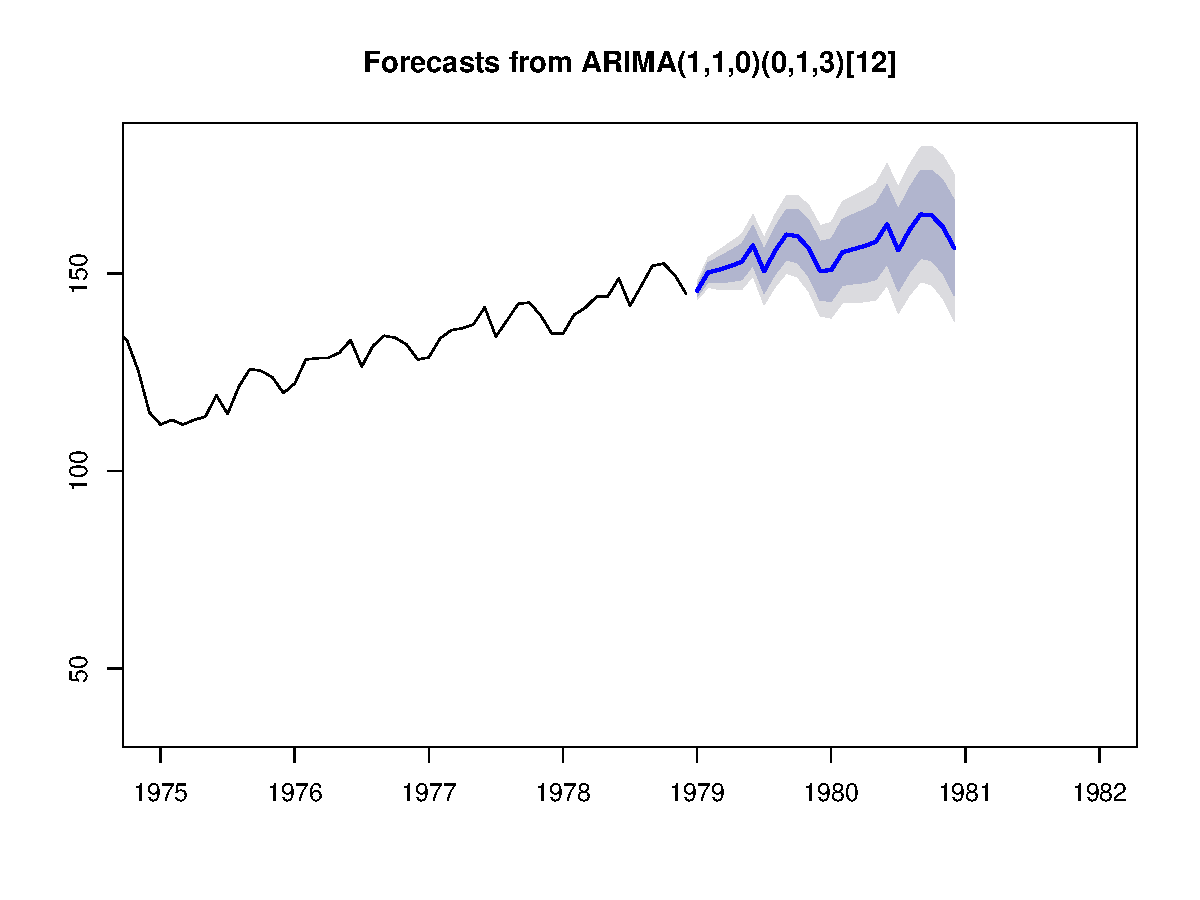
\includegraphics{Lec11_files/figure-beamer/unnamed-chunk-27-1.pdf}

\end{frame}

\begin{frame}{Model Forecast (cont.)}

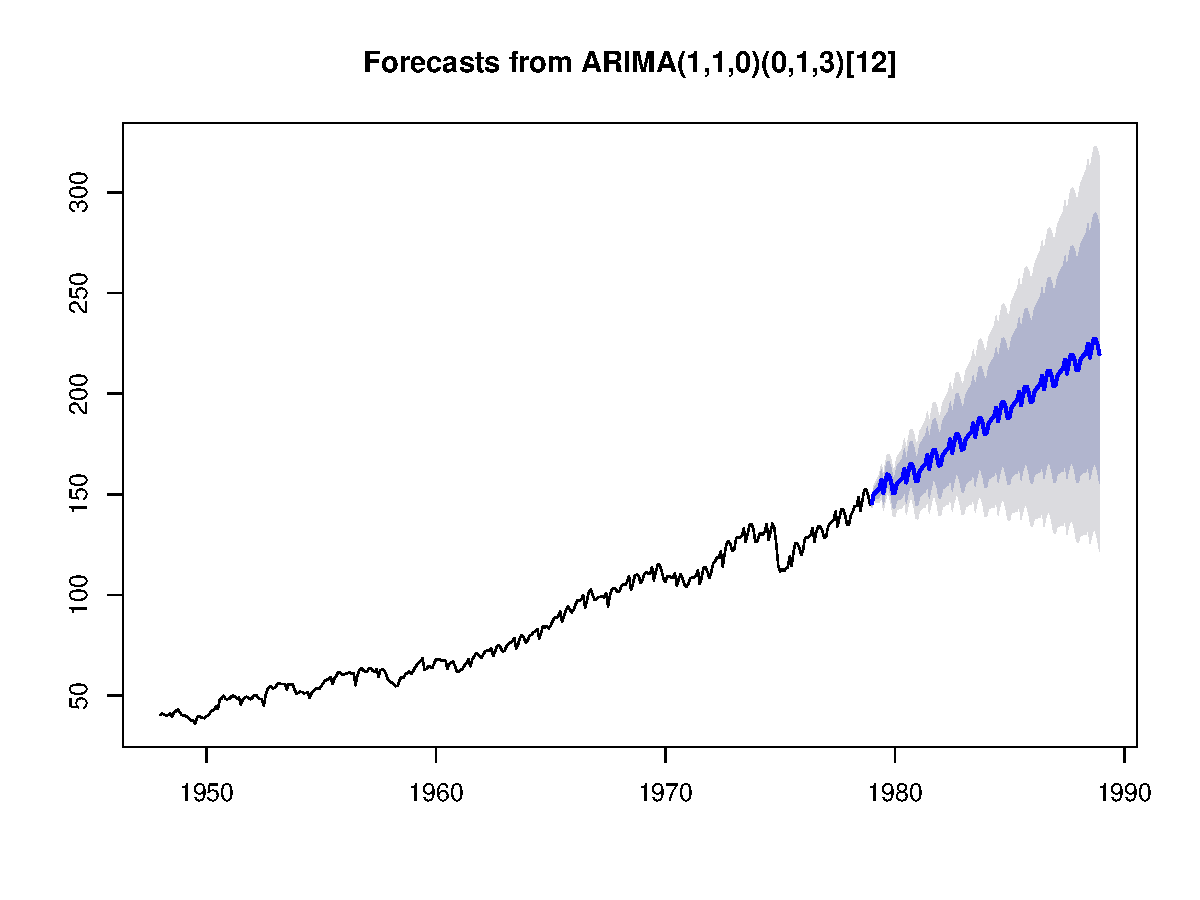
\includegraphics{Lec11_files/figure-beamer/unnamed-chunk-28-1.pdf}

\end{frame}

\begin{frame}{Model Forecast (cont.)}

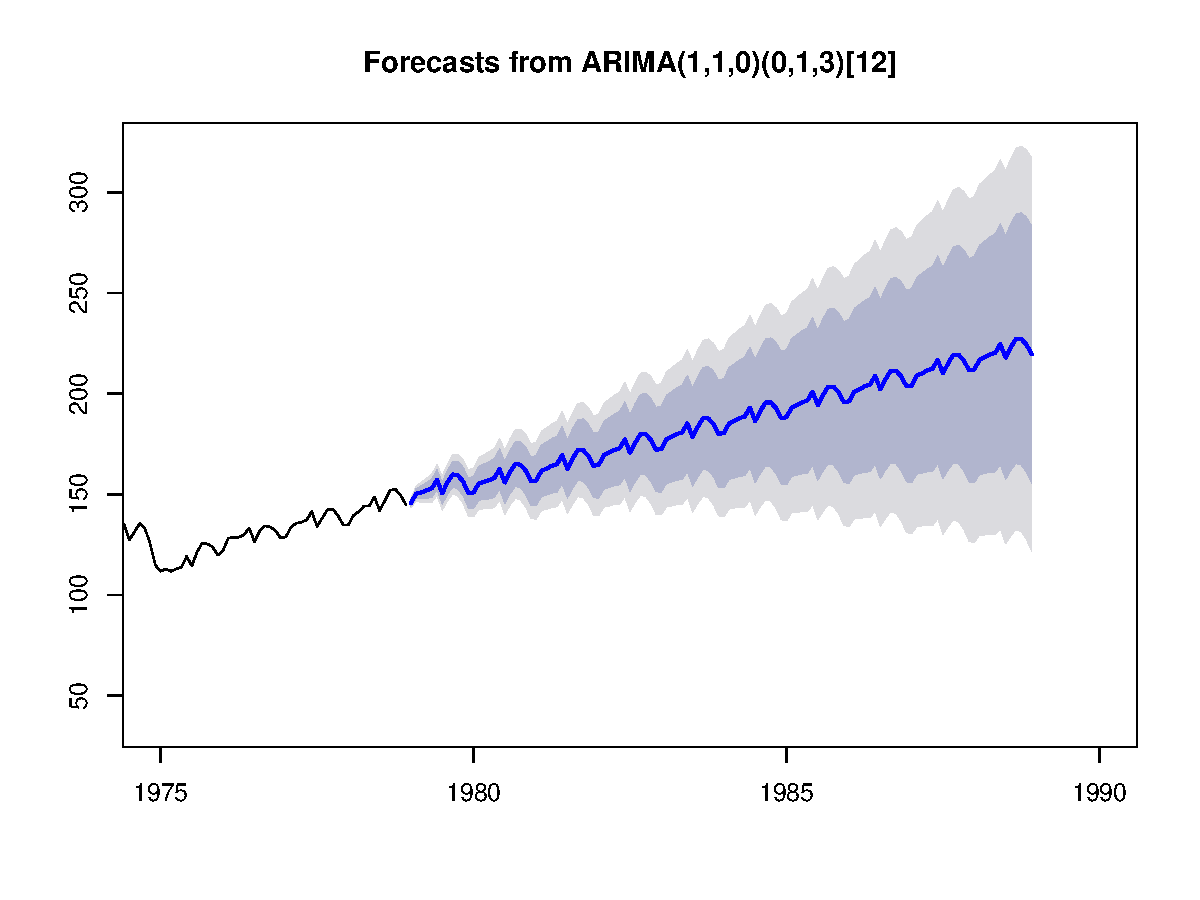
\includegraphics{Lec11_files/figure-beamer/unnamed-chunk-29-1.pdf}

\end{frame}

\begin{frame}[fragile]{Exercise - Cortecosteroid Drug Sales}

Monthly cortecosteroid drug sales in Australia from 1992 to 2008.

\begin{Shaded}
\begin{Highlighting}[]
\KeywordTok{library}\NormalTok{(fpp)}
\KeywordTok{tsdisplay}\NormalTok{(h02,}\DataTypeTok{points=}\OtherTok{FALSE}\NormalTok{)}
\end{Highlighting}
\end{Shaded}

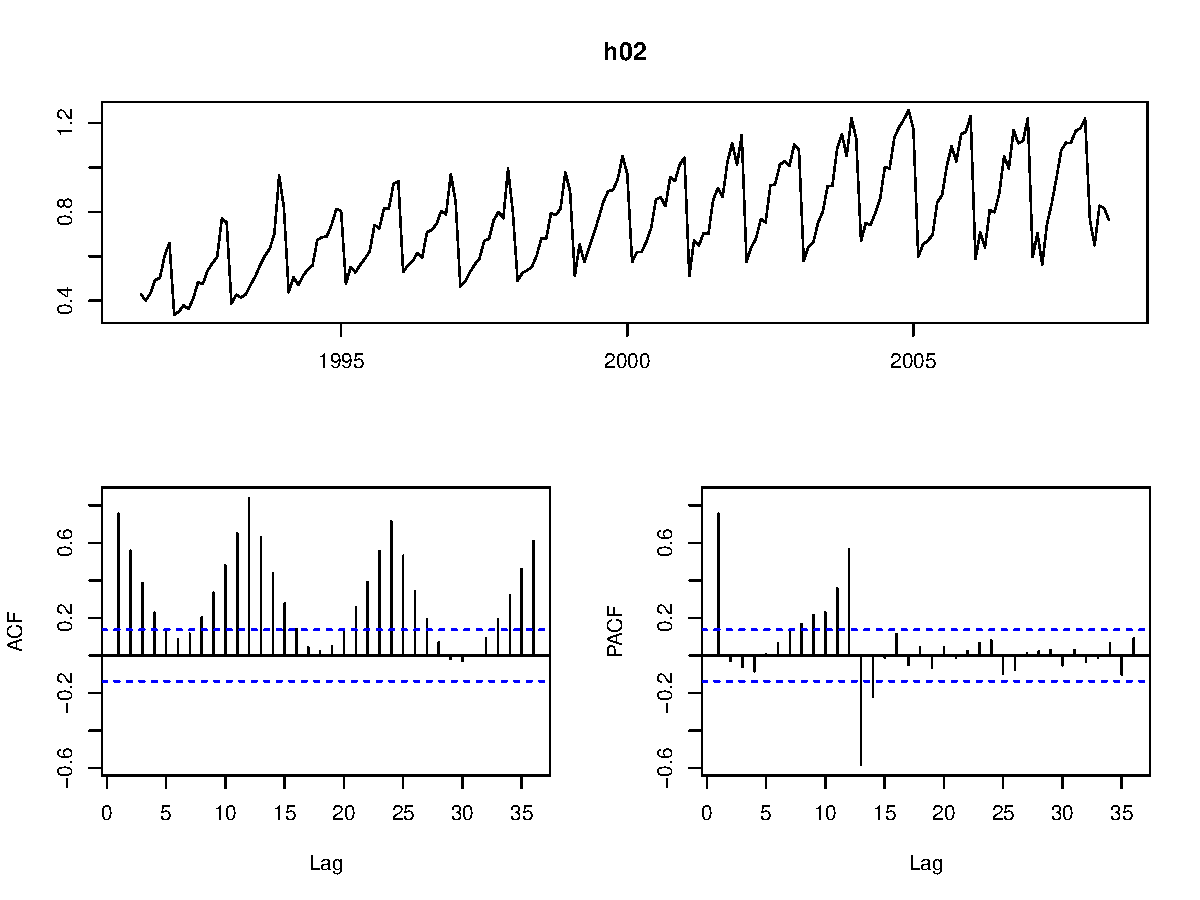
\includegraphics{Lec11_files/figure-beamer/unnamed-chunk-30-1.pdf}

\end{frame}

\begin{frame}[fragile]{Hint}

\begin{Shaded}
\begin{Highlighting}[]
\KeywordTok{ts.intersect}\NormalTok{(h02, }\KeywordTok{log}\NormalTok{(h02)) }\OperatorTok\StringTok{ }\KeywordTok{plot}\NormalTok{()}
\end{Highlighting}
\end{Shaded}

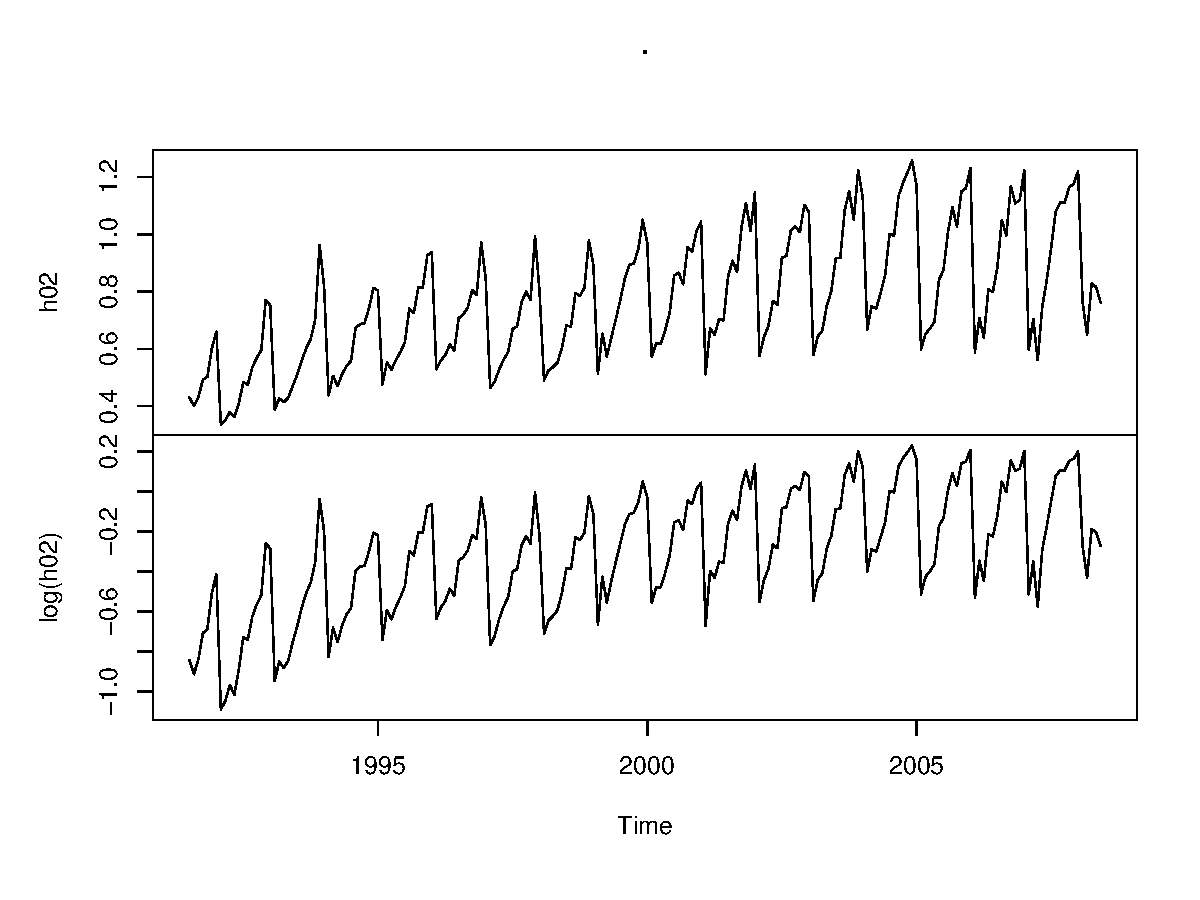
\includegraphics{Lec11_files/figure-beamer/unnamed-chunk-31-1.pdf}

\end{frame}

\end{document}
